% !TeX spellcheck = ru_RU
\chapter{Определение позы человека в видеопоследовательности} \label{chapt6}

В этой главе я рассматриваю задачу определения позы человека в видеопоследовательности. Как описано в обзоре \ref{chapt-related::human_pose_definithion}, в настоящий момент научное сообщество определяет позу человека на изображении как положение его $K$ суставов. Таким образом, позой человека в момент времени $t$ является последовательность точек $P^t \in \left\{ \left\{p_i^t\right\}_{i=1}^K | p_i^t \in \mathbb{R}^2\right\}$ на изображении.

В своей работе я рассматриваю алгоритм определения позы человека в качестве следующего этапа обработки видеоданных после сопровождения. Поэтому моя постановка задачи определения позы в видеопоследовательности имеет следующий вид:
\begin{itemize}
	\item[Вход:] видеопоследовательность $I=\left\{I_t\right\}_{i=1}^N$;
	\item[Выход:] поза человека на каждом кадре $P=\left\{P^t\right\}_{t=1}^{N}$.
\end{itemize}

\section{Математическая модель наблюдаемых данных}

Я рассматриваю определение позы человека в видео как задачу минимизации функции энергии $E(P, \Theta|I)$, где $\Theta$ "--- скрытые параметры модели. Параметр $\Theta$ может включать как скрытые параметры позы человека на одно кадре (например, параметр размера), так и глобальные параметры модели человека (цветовая модель). Можно считать, что функция энергии $E(P, \Theta|I)$ задаёт ненормированную функцию правдоподобия позы в видеопоследовательности в виде $\tilde{p}(P, \Theta|I) = \exp\left(-E(P, \Theta|I)\right)$. В дальнейшем для упрощения выкладок я буду неявно предполагать зависимость функции энергии от исходной видеопоследовательности, т.~е. $E(P, \Theta) = E(P, \Theta|I)$.

Используемая модель наблюдаемых данных является обобщением модели позы человека на изображении на случай видеопоследовательности. Для этого базовая модель расширяется предположением о зависимости позы человека на разных кадрах. Стандартный подход к расширению модели позы человека на случай видеопоследовательности соответствует следующей функции энергии:
\begin{equation}
	\begin{aligned}
		E(P, \Theta) &= \sum_{t=1}^T E_I(P^t, \Theta) + \sum_{t=1}^{T-1}E_T(P^{t+1}, P^{t}, \Theta),
	\end{aligned}
\end{equation}
где $E_I(P^t)$ "--- модель позы человека на кадре \eqref{eq::frame}, а $E_T(P^{t+1}, P^{t})$ "--- модель изменения позы между кадрами. Такую модель можно рассматривать как марковскую цепь первого порядка, где состояние в каждый момент времени является многомерной величиной и описывает позу человека.

Она состоит из двух частей: 1) базовая модели позы человека на изображении $E_I(P^t, \Theta)$ и 2) модель движения её суставов $E_T(P^{t+1}, P^{t}, \Theta)$.

\subsection{Модель позы человека на изображении}

Согласно обзору существующих методов в научных работах представлены две основные модели позы человека: модель из набора деформируемых частей и регрессионная модель позы.

Несмотря на то, что регрессионная модель на момент написания данной диссертации позволяет добиться лучших результатов определения позы на изображении, её обобщение на случай видеопоследовательности затруднено. Построенное отображение входного изображения $I_t$ на позу человека $P^t$ на нем не позволяет использовать априорные сведения, полученные на соседних кадрах.

Поэтому в качестве базовой модели позы человека на изображении была выбрана модель из набора деформируемых частей. Соответствующая ей марковская сеть, определяет ненормированную функцию правдоподобия $\tilde{p}(P^t, \Theta^t) = \exp(-E_I(P^t, \Theta))$. Это свойство позволяет интегрировать её как часть большей графической модели, используя информацию с предыдущих кадров для построения априорных ограничений.

Модель из набора частей описывается с помощью функции энергии $E_I(P^t, \Theta^t)$, минимум которой определяется в качестве позы человека на изображении $I_t$:
\begin{equation}
	E_I(P^t, \Theta) = \sum_{i=1}^K{\phi_i(p_i^t, s^t)} + \sum_{\left(i,j\right)\in E}{\psi_{(i,j)}^s(p_i^t, p_j^t, s^t)},
	\label{eq::frame}
\end{equation}

Унарный потенциал $\phi_i(p_i^t, s^t)$ можно рассматривать, как отклик алгоритма обнаружения сустава человека на заданном масштабе изображения. Парный потенциал $\psi_{(i,j)}^s(p_i^t, p_j^t, s^t)$ задаётся в виде квадратичной формы, зависящей от смещения между суставами. Функция энергии зависит от параметра размера человека $s^t$ на текущем изображении, и не зависит от остальных скрытых параметров модели.

На практике параметр положения $p^t$ суставов является дискретной величиной, определённой на изображении с некоторым шагом. Параметр размера $s^t$ также является дискретным и соответствует разным масштабам при обнаружении суставов.

\subsection{Модель движения}

Наиболее простым способом задания модели изменения позы является предположение о независимости движения суставов:
\begin{equation}
	E_T(P^{t+1}, P^{t}, \Theta) = \sum_{i=1}^K\psi_i^t(p_i^{t+1}, p_i^t, \Theta)
\end{equation}

Так как модели движения разных суставов схожи, то достаточно рассмотреть её лишь для одного из них. Для упрощения обозначений в данном подразделе я опускаю индекс рассматриваемого сустава. Например, $p^t$ используется для обозначения состояния рассматриваемого сустава на кадре $I_t$.

Такое расширение модели позы человека на изображении на случай видеопоследовательности использовался также в предыдущих работах. Например, в работе \cite{park2011n} предлагалась модель движения, предполагающее слабое изменение позы человека между кадрами:
\begin{equation*}
	\psi^t(p^{t+1}, p^t, \Theta) = \frac{1} {2 {s^t}^2}(p^{t+1} - p^t)^{T-1} \left(\Sigma_p^p\right)^{-1} (p^{t+1} - p^t)
\end{equation*}
Таким образом, оптимальное значение такой модели движения достигается при постоянстве позы человека в видео. Изменение позы при движении оказывается <<допустимым шумом>>.

В этой работе я расширил эту модель движения. Я использовал линейную динамическую систему для описания движения суставов тела человека. Для этого скрытое состояние $\Theta$ модели было расширено характеристикой движения каждого сустава. В работе я рассматриваю линейную модель движения суставов, т.~e. состояние каждого сустава описывается его положением $p^t$ на кадре и мгновенной скоростью движения $v^t \in \mathbb{R}^2$. По аналогии с позой человека, я обозначаю скорость всех суставов в видеопоследовательности через $V$. Если обозначить через $h^t = [p^t, v^t]$ "--- состояние рассматриваемого сустава позы человека на кадре $t$, то предложенная модель движения принимает вид:
\begin{equation}
	\begin{aligned}
		\psi^t(p^{t+1}, p^{t}, \Theta) &=
			\frac{1}{2 {s^t}^2} (h^{t+1} - A h^t)^T \Sigma_p^{-1} (h^{t+1} - A h^t) \\
		A &=
			\begin{bmatrix}
			1 & 0 & 1 & 0 \\
			0 & 1 & 0 & 1 \\
			0 & 0 & 1 & 0 \\
			0 & 0 & 0 & 1 \\
			\end{bmatrix} \\
	\label{eq::temp}
	\end{aligned}
\end{equation}

Допустимое отклонение от линейной модели движения задается симметричной положительно определенной матрицей $\Sigma_p \in \mathbb{S_+}$. Для уменьшения количества параметров я рассматривал только диагональные матрицы $\Sigma_p$ следующего вида:
\begin{equation}
	\begin{aligned}
		\Sigma_p &= \left[
			\begin{array}{c|c}
			\Sigma_p^p & \Theta \\ \hline
			\Theta     & \Sigma_p^v
			\end{array}
			\right] \\
		\Sigma_p^p &= \alpha_p^{-1} I_{2\times2} \\
		\Sigma_p^v &= \alpha_v^{-1} I_{2\times2} \\
		\alpha_p &> 0, \alpha_v > 0,
		\label{eq::sigma}
	\end{aligned}
\end{equation}
Матрица $\Sigma_p^p$ описывает допустимое отклонение положения сустава $p^{t+1}$ от его линейного предсказания $p^t + v^t$, a $\Sigma_p^v$ "--- допустимое изменение скорости сустава между кадрами.

Без дополнительной регуляризации модель движения \eqref{eq::temp} допускает неправдоподобно большое значение скорости движения сустава, так как ограничивает только её изменение. Для решения этой проблемы был добавлен фактор, задающий априорное предпочтение на скорость движения суставов на первом кадре:
\begin{equation}
	\begin{aligned}
		\psi^0(v^1) &= \frac{1}{2 {s^1}^2}{v^1}^T \left({\Sigma_p^{v^1}}\right)^{-1} v^1 \\
		\Sigma_p^{v^1} &= \alpha_{v^1}^{-1} I_{2\times2}
	\end{aligned}
\end{equation}

Также моя модель ограничивает неправдоподобное изменение размера человека между кадрами:
\begin{equation}
	\eta^t(s^{t+1}, s^t) = \frac{1}{2} \left(\frac{s^{t+1} - s^t}{s^t\sigma_s}\right)^2
\end{equation}

Таким образом, предложенная модель движения имеет следующий вид:
\begin{equation}
	\sum_{t=1}^{T-1}{\Psi(P^{t+1}, P^t)} = 
		\sum_{i=1}^K\left(\psi^0_i(v^1_i) + \sum_{t=1}^{T-1}\psi_i^t(h_i^{t+1}, h_i^{t}, \Theta) \right) + \sum_{t=1}^{T-1} \eta^t(s^{t+1}, s^{t})
	\label{eq::motion_model}
\end{equation}

\subsection{Частные случаи}

Предложенная модель имеет два интересных частных случая, рассматриваемых в предыдущих работах.

Рассмотрим случай, когда $\alpha_v \rightarrow +\infty, \alpha_{v^1} \rightarrow +\infty$ и $\sigma_s \rightarrow +\infty$. Этот случай описывает значительное увеличение энергии в случаях, когда значение скорости какого-либо сустава отлично от $0$:
\begin{equation}
	\begin{aligned}
		\lim_{\alpha_{v^1} \rightarrow +\infty}{\argmin_{v^1} \psi^0(v^1)} &= 0 \\
		\lim_{\alpha_{v} \rightarrow +\infty}{\argmin_{v^t} \psi^t(h_i^{t+1}, h_i^{t}, \Theta)} &= 0 \\
		\lim_{\sigma_s \rightarrow +\infty}{\eta^t(s^{t+1},s^t)} &= 0
	\end{aligned}
\end{equation}
То есть оптимальным является решение, где все параметры скорости равны 0. При этом условии модель движения суставов имеет вид:
\begin{equation}
	\begin{aligned}
		\psi^t(h_i^{t+1}, h_i^{t}, \Theta) |_{v^t = v^{t+1} = 0} &= \frac{1} {2 {s^t}^2}(p^{t+1} - p^t)^T \left(\Sigma_p^p\right)^{-1} (p^{t+1} - p^t) \\
		\psi^0(v^1)|_{v^1=0} &= 0
	\end{aligned}
\end{equation}
То есть предложенная модель становится эквивалентной модели движения, описанной в работе \cite{park2011n}.

Рассмотрим другой частный случай. Если ослабить ограничения на небольшое изменение скорости суставов между кадрами, то модель \eqref{eq::motion_model} описывает независимое определение позы человека на каждом кадре. Действительно
\begin{equation}
	\begin{aligned}
		\lim_{\alpha_{v} \rightarrow 0+0}{\psi^t(h_i^{t+1}, h_i^{t}, \Theta)} &= 0 \\
		\lim_{\alpha_{v^1} \rightarrow 0+0}{\psi^0(v^1)} &= 0 \\
		\lim_{\sigma_s \rightarrow +\infty}{\eta^t(s^{t+1},s^t)} &= 0
	\end{aligned}
\end{equation}
То есть графическая модель распадается на независимые связные компоненты, соответствующие позе человека на каждом кадре.

\section{Метод оптимизации}

\subsection{Анализ модели}

\label{subsec::model_analysis}

Для описания предложенного алгоритма оптимизации важно рассмотреть две задачи, связанные с функцией представленной функции энергии:
\begin{enumerate}
	\item определение скорости суставов при известных позе и росте человека человека в видео "--- $\argmin_{V} E(P, \Theta)$;
	\item определение позы и размера человека на кадре $t$ при известных остальных параметрах модели "--- $\argmin_{P^t, s^t} E(P, \Theta)$.
\end{enumerate}

\subsubsection{Определение скорости}

\begin{figure*}[!t] 
	\begin{center}
		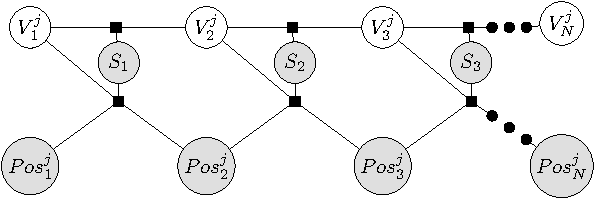
\includegraphics{human_pose/5.pdf}
		%		%\beginpgfgraphicnamed{model-simpleModel}
\begin{tikzpicture}

\tikzstyle{myDot} = [circle, fill=black,minimum size=5pt, inner
sep=0pt]

  % Define nodes
  \node[obs]                                  (P1) {$POS_1^j$};
  \node[obs, right=2cm of P1]                 (P2) {$POS_2^j$};
  \node[obs, right=2cm of P2]                 (P3) {$POS_3^j$};
  \node[obs, right=2cm of P3]                 (PN) {$POS_N^j$};
  \node[obs, above=0.9cm of P1, xshift=1.5cm] (S1) {$S_1$};
  \node[obs, above=0.9cm of P2, xshift=1.5cm] (S2) {$S_2$};
  \node[obs, above=0.9cm of P3, xshift=1.5cm] (S3) {$S_3$};
  \node[latent, above=1.5cm of P1]            (V1) {$V_1^j$};
  \node[latent, above=1.5cm of P2]            (V2) {$V_2^j$};
  \node[latent, above=1.5cm of P3]            (V3) {$V_3^j$};
  \node[latent, above=1.5cm of PN]            (VN) {$V_N^j$};
  \node[myDot, right=1.4cm of V3]             (Dot1) {};
  \node[myDot, right=0.10cm of Dot1]          (Dot2) {};
  \node[myDot, right=0.10cm of Dot2]          (Dot3) {};
  \node[myDot, right=1.4cm of V3, yshift=-1.5cm]    (Dot21) {};
  \node[myDot, right=0.10cm of Dot21, yshift=-0.2cm]  (Dot22) {};
  \node[myDot, right=0.10cm of Dot22, yshift=-0.2cm]  (Dot23) {};

  % unary factors
  \factor [below=0.8cm of V1, xshift=1.5cm] {V1-factor}  {} {} {}
  \factor [below=0.8cm of V2, xshift=1.5cm] {V2-factor}  {} {} {}
  \factor [below=0.8cm of V3, xshift=1.5cm] {V3-factor}  {} {} {}
  % pairwise factors
  \factor [right=1cm of V1] {V12-factor}  {} {} {}
  \factor [right=1cm of V2] {V23-factor}  {} {} {}
  \factor [right=1cm of V3] {V3N-factor}  {} {} {}

  %% Connect the nodes
  % unary
  \factoredge {P1, P2, V1, S1} {V1-factor} {}
  \factoredge {P2, P3, V2, S2} {V2-factor} {}
  \factoredge {P3, Dot21, V3, S3} {V3-factor} {}
  \draw (Dot23) -- (PN);
  % paiwise
  \factoredge {V1, V2, S1} {V12-factor} {}
  \factoredge {V2, V3, S2} {V23-factor} {}
  \factoredge {V3, Dot1, S3} {V3N-factor} {}
  \draw (Dot3) -- (VN);

  % Plates
%  \plate {yx} {(x)(y)} {$N$} ;
%  \plate {} {(w)(y)(yx.north west)(yx.south west)} {$M$} ;

\end{tikzpicture}
%\endpgfgraphicnamed
	\end{center}
	\caption{Фактор граф, соответствующий задаче определения скорости. Наблюдаемые переменные отмечены серым} \label{gm:velocity}
\end{figure*}

Рассмотрим задачу определение скорости движения суставов при известных позе и росте человека в видео $V = \argmin_{V} E(P, \Theta)$. Модель позы человека на изображении $E_I(P^t, \Theta)$ и модель изменения размера $\eta^t(s^{t+1}, s^t)$ не зависят от параметров скорости. Поэтому рассматриваемая задача эквивалентна задаче оптимизации:
\begin{equation}
	V = \argmin_V E(V|P, \Theta_{\backslash V}) = \argmin_V {\sum_{i=1}^K\left(\psi^0_i(v^1_i) + \sum_{t=1}^{T-1}\psi_i^t(h_i^{t+1}, h_i^{t}, \Theta) \right)}
\end{equation}
Из этой формы видно, что скорости разных суставов никогда не входят в одно слагаемое, а значит можно проводить оптимизацию скорости каждого сустава независимо:
\begin{equation}
	\begin{aligned}
		V_i &= \argmin_{V_i} \psi^0_i(v^1_i) + \sum_{t=1}^{T-1}\psi_i^t(h_i^{t+1}, h_i^{t}, \Theta) \\
		V &= \cup_{i=1}^K V_i
	\end{aligned}
\end{equation}

Рассмотрим поиск оптимального значения для скорости одного сустава. В дальнейшем для упрощения выкладок я буду опускать индекс текущего сустава. Функции энергии $E(V|P, \Theta_{\backslash V})$ соответствует фактор граф на рисунке \ref{gm:velocity}. Можно заметить, что соответствующая графическая модель является марковской цепью первого порядка. Учитывая \eqref{eq::temp} и \eqref{eq::sigma}, оптимизируемую энергию $E(V|P, \Theta_{\backslash V})$ можно переписать в виде суммы унарных и парных потенциалов:
\begin{equation}
	\begin{aligned}
		E(V|P, \Theta_{\backslash V}) &= \psi^0(v^1) + \sum_{t=1}^{T-1} \left( \psi^{t,u}(v^t|p^{t+1}, p^{t}, s^t) + \psi^{t,p}(v^{t+1}, v^{t}|s^t) \right) \\		
		\psi^{t,u}(v^t|p^{t+1}, p^{t}, s^t) &= \frac{(\Delta p^t - A^u v^t)^T {\Sigma_p^p}^{-1} (\Delta p^t - A^u v^t)} {2 {s^t}^2} \\
		\psi^{t,p}(v^{t+1}, v^{t}|s^t) &= -\frac{(v^{t+1} - A^p v^t)^T {\Sigma_p^v}^{-1} (v^{t+1} - A^p v^t)} {2 {s^t}^2} \\ 
		\Delta p^t &= p^{t+1} - A_p^u p^t \\
		A &= \left[
		\begin{array}{c|c}
		A_p^u  & A^u \\ \hline
		\Theta & A^p
		\end{array}
		\right] \quad
		A_p^u, A^u, A^p \in \mathbb{R}^{2 \times 2}
	\end{aligned}
\end{equation}

В данной постановке задача поиска минимума функции энергии $E(V|P, \Theta_{\backslash V})$ совпадает с задачей определения состояний линейной динамической системы (ЛДС):
\begin{equation}
\begin{aligned}
	V &= \argmax_V {p\left(V | \left\{\Delta p^t\right\}_{t=1}^{T-1}, \left\{s^t\right\}_{t=1}^T\right)} \\ 
	\Delta p^t &\sim N(A^u v^t, (s^t)^2\Sigma_p^p) \\
	v^{t+1} &\sim N(A^p v^t, (s^t)^2\Sigma_p^v) \\
	v^1 &\sim N(\Theta, (s^t)^2\Sigma_p^{v^1}) \\
	v^T &= A^p v^{T-1}
\end{aligned}
\end{equation}
Поиск наиболее вероятной конфигурации $V$ осуществляется с помощью фильтра Калмана и РТС уравнений.

\subsubsection{Определение позы и размера на кадре}

\begin{figure}[t]
	\begin{center}
		\begin{tabular}{cc}
			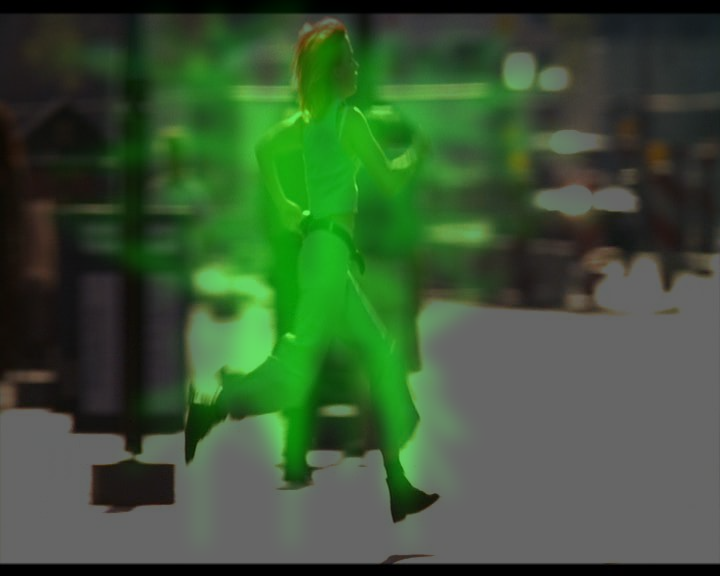
\includegraphics[width=62mm]{human_pose/7.png} & 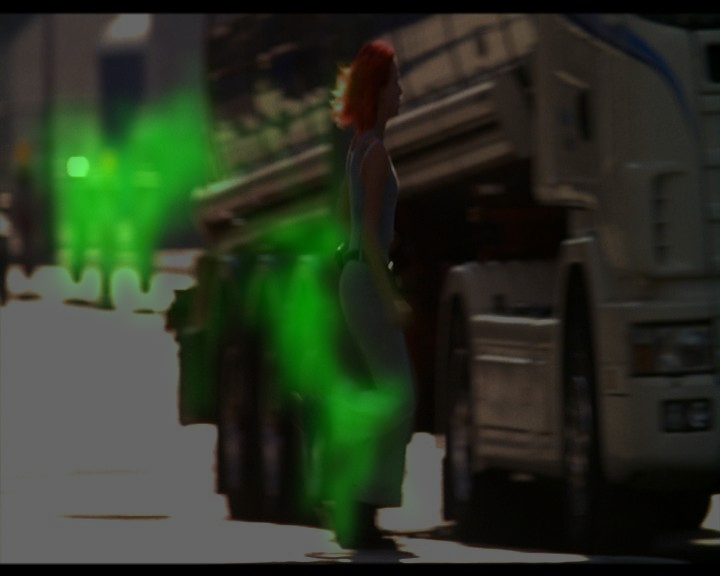
\includegraphics[width=62mm]{human_pose/8.png} \\
			(а) & (б)
		\end{tabular}
		\caption{Визуализация наилучших гипотез позы человека на кадре. Интенсивность зелёной подсветки соответствует количеству построенных гипотез позы человека На кадре (а) большинство обнаруженных гипотез близки к верной позе человека. На кадре (б) детектор не смог найти хорошее множество гипотез позы человека.}
		\label{fig:good_bad_hypotheses}
	\end{center}
\end{figure}

Рассмотрим задачу определения позы $P^t$ и размера $s^t$ человека на некотором кадре при известных остальных параметрах модели $\argmin_{P^t, s^t} E(P, \Theta)$:
\begin{multline}
	E(P^t, s^t| P^{\backslash t}, \Theta_{\backslash s^t}) = E(P, \Theta)\bigg\rvert_{P^{\backslash t}, \Theta_{\backslash s^t}} = \\ = \left(\sum_{t'=1}^T{E_I(P^{t'}, \Theta)} + \sum_{t'=1}^{T-1}{E_T(P^{t'+1}, P^{t'}, \Theta)}\right)\bigg\rvert_{P^{\backslash t}, \Theta_{\backslash s^t}}
\end{multline}

Модель позы человека в видео является марковской цепью первого порядка, поэтому рассматриваемая энергия имеет вид:
\begin{multline}
	E(P^t, s^t| P^{\backslash t}, \Theta_{\backslash s^t}) = E_I(P^{t}, \Theta) + \\ + \left(E_T(P^{t+1}, P^{t}, \Theta) + E_T(P^{t}, P^{t-1}, \Theta)\right)\bigg\rvert_{\substack{P^{t-1}, P^{t+1}, \\ s^{t-1}, s^{t+1}, \\ V^{t-1}, V^{t+1}}} + C,
\end{multline}
где $C$ "--- константа, не зависящая от рассматриваемых параметров. Чтобы не рассматривать отдельно случаи граничные случаи, можно определить состояние модели в моменты времени $t=0$ и $t=T+1$ значениями в моменты времени $t=1$ и $t=T$ соответственно.

Учитывая \eqref{eq::frame} и \eqref{eq::temp}, рассматриваемая энергия имеет вид:
\begin{multline}
	E(P^t, s^t| P^{\backslash t}, \Theta_{\backslash s^t}) =
	 \sum_{i=1}^K{
	 	\left(\underbrace{\phi_i(p_i^t, s^t) +
	 		 \psi_i^t(h_i^{t+1}, h_i^{t}, \Theta) +
	 		 \psi_i^t(h_i^{t}, h_i^{t-1}, \Theta)}_{\phi'_i(p_i^t, s^t)} \right)} + \\ +
 		  \sum_{\left(i,j\right)\in E}{
 		  	\psi_{(i,j)}^s(p_i^t, p_j^t, s^t)} +
 	  	  \underbrace{\eta^t(s^{t+1}, s^{t}) + \eta^t(s^{t}, s^{t-1}) + C'}_{\phi_s(s^t)}
\end{multline}

Таким образом, условная модель человека $E(P^t, s^t| P^{\backslash t}, \Theta_{\backslash s^t})$ на кадре $I_t$ для каждого масштаба $s^t$ представляет сумму унарных $\phi'_i(p_i^t, s^t)$ и парных $\psi^s_{(i,j)}(p_i^t, p_j^t, s^t)$ потенциалов относительно положения суставов позы человека. Так как модель движения не добавляет парных потенциалов в энергию $E(P^t, s^t| P^{\backslash t}, \Theta_{\backslash s^t})$, то эта энергия факторизуется согласно той же графической модели, что и модель позы $E_I(P^t, \Theta)$. Факторы $\eta^t(s^{t+1}, s^t)$ и $\eta^t(s^t, s^{t-1})$ задают апостериорное предпочтение на значение параметра размера позы.

Таким образом, условная модель позы человека $E(P^t, s^t| P^{\backslash t}, \Theta_{\backslash s^t})$ является обобщением модели позы человека на изображении $E_I(P^t, \Theta)$. Так как при оптимизации модели $E_I(P^t, \Theta)$ алгоритмы производят перебор по различным значениям параметра размера человека $s^t$, то для условной модели позы человека также выполняются свойства:
\begin{enumerate}
	\item вычислительная сложность алгоритма поиска глобального оптимума равна $\mathcal{O}(KM)$;
	\item алгоритм построения множества наилучших гипотез позы человека на изображении, отличающихся не менее чем на заданную величину равна имеет сложность $\mathcal{O}(KM)$.
\end{enumerate}

На рисунке \ref{fig:good_bad_hypotheses} показан пример множества наилучших гипотез позы человека на изображении в ситуации, когда детектор верно локализует суставы и не может корректно определить позу человека.

\subsubsection{Сложность поиска глобального оптимума}

Каждой функции энергии, описывающей модель позы человека, соответствует марковская сеть. От её свойств зависит сложность алгоритмов поиска оптимального значения модели. В общем случае поиск глобального оптимума в графических моделях осуществляется алгоритмом распространения доверия. Его вычислительная сложность зависит от количества допустимых состояний минимальной группы вершин, разделяющих графическую модель на две части. Если графическая модель является деревом, то сложность алгоритма квадратично зависит от количества допустимых состояний для каждой вершины. Примером такой графической модели является модель позы человека на изображении при условии известного параметра масштаба. Специальный вид парных потенциалов, позволил сократить сложность вывода в графической модели до линейной зависимости от количества допустимых положений суставов на изображении.

К сожалению, при расширении этой модели, в марковской сети появляются циклы, а следовательно сложность поиска оптимального решения существенно возрастает. На рисунке \ref{} представлена графическая модель, соответствующая модели \cite{park2011n}. Её можно рассматривать как марковскую цепь первого порядка, где каждое состояние описывается множеством вершин одного кадра.

Рассмотрим вычислительную сложность алгоритма поиска глобального минимума для такой марковской цепи. Если на кадре имеется $M$ возможных положений каждого сустав, то сложность алгоритма распространения доверия равна $\mathcal{O}(M^{K}T)$. Здесь существенно использован факт, что модель движения \eqref{eq::motion_model} является квадратичной формой, и для вычисления сообщений в сети может быть использован метод дистантного преобразования. Таким образом, сложность поиска оптимального множества поз линейно зависит от количества возможных поз человека на изображении. Так как значение параметра $M$ может превосходить $10^4$, а количество суставов исчисляться десятками, то алгоритм поиска точного решения оказывается не применим на практике. Уменьшив количество допустимых поз на кадре изображения, авторы \cite{park2011n} построили алгоритм поиска локального оптимума со сложностью $\mathcal{O}(HT)$, где $H$ "--- количество допустимых поз на одном кадре.

Предложенная в данной работе модель является расширением \cite{park2011n} и содержит её в качестве частного случая. Алгоритм распространения правдоподобия не может быть применён для поиска глобального оптимума предложенной модели, так как потребует слишком больших вычислительных ресурсов. Также скрытое состояние $\Theta$ дополнительно содержит непрерывные параметры скорости суставов, то есть описанная модель является дискретно-непрерывной. Это не позволяет использовать алгоритм \cite{park2011n} напрямую. Я предложил два алгоритма поиска оптимального значения построенной функции энергии. Первый алгоритм использует идею работы \cite{park2011n} для поиска локального оптимума, а второй "--- метод построения выборки из распределения для уточнения результата.

\begin{algorithm}[t]
	\SetAlgoLined %% Это соединяет линиями логические части 
	%% алгоритма типа if-then-else
	
	\KwData{ $I, N$} %% здесь можно указать исходные параметры
	
	\KwResult{ $P$ } %% результат работы программы
	
	$r \leftarrow \max(I.width(), I.height())$;
	
	$P \leftarrow N\_best(E(P, \Theta)\bigg\rvert_{V=0},N, r)$;
	
	$V \leftarrow \argmin_V{E(V|P, \Theta_{\backslash V})}$;
	
	\While{ $r > 1$ }{
		
		$E_0 \leftarrow E(P,\Theta)$;
		
		\For{$t=\overline{1,T})$} {
		
		$\left\{\left(\overline{P}_k^t, \overline{s}_k^t \right)\right\}_k \leftarrow N\_best\left(E(P^t, s^t | P_{\setminus t}, \Theta_{\backslash s^t}), N, r \right)$;
		
		\For{$k=\overline{1,K}$}{
			
			$\overline{P}_k \leftarrow \left\{P_{\setminus t}, \overline{P_k^t} \right\}$
			
			$\overline{\Theta}_k \leftarrow \left\{\Theta, \overline{s}^t_k\right\}$
			
			$\overline{V}_k \leftarrow \argmin_V {E(V|\overline{P}_k, {\overline{\Theta}_{k,\backslash V}})}$;
		}
		
		$\left(P, \Theta\right) \leftarrow \argmin_{\overline{P}_k, \overline{\Theta}_k}{\left\{E(\overline{P}_k, \overline{\Theta}_k)\right\}}$;
		}
		\If{$E(P, \Theta) = E_0$}{
			
			$r \leftarrow \frac{r}{2}$;
			
		}

	}
	
	\caption{Итеративный алгоритм построения позы человека в видео.}
	\label{alg:generalInit}
\end{algorithm}

\subsection{Детерминированный алгоритм}

Рассмотрим первый из предложенных алгоритмов. Его псевдокод представлен на листинге \ref{alg:generalInit}. 

Идея алгоритма основана на последовательном решении двух задач: 1) построение гипотез позы человека на кадре согласно условной модели позы $E(P^t, s^t| P^{\backslash t}, \Theta_{\backslash s^t})$; 2) вычисление оптимального значения параметра скорости, согласно модели $E(V|P, \Theta_{\backslash V})$. Способ решения этих задач описан в разделе \ref{subsec::model_analysis}.

Для построения начальной инициализации я использую метод, предложенный в работе \cite{park2011n}, то есть минимизируется энергия модели при условии, что скорость движения суставов равна нулю $E(P, \Theta)\bigg\rvert_{V=0}$. Для построенного приближенного решения позы и размера человека оценивается скорость движения суставов путём минимизации $E(V|P, \Theta_{\backslash V})$.

После этого итеративно до сходимости предложенный алгоритм выбирает произвольный кадр видеопоследовательности и улучшает оценку позы и скрытых параметров, ассоциированных с этим кадром. Согласно разделу \ref{subsec::model_analysis}, для произвольного кадра можно определить оптимальную позу и параметр размера на нём, если остальные параметры модели известны. Однако, для выбранного кадра $I_t$ оценка скорости, полученная на предыдущем шаге может быть неоптимальной. Поэтому в предложенном алгоритме происходит построение набора из $N$ гипотез позы человека. Для каждой из них определяется значение параметров скорости, и выбирается гипотеза приводящая к наибольшему уменьшению функции энергии.

Метод построения гипотез позы человека на изображении, предложенный в работе \cite{park2011n}, зависит от двух гиперпараметров: 1) радиуса $r$, определяющего минимальное различие между построенными гипотезами и 2) количества гипотез $N$, которое необходимо построить. Большое значение радиуса $r$ позволяет получить существенно отличающиеся гипотезы позы и подходит для работы в случае неверно определённого значения скорости. Малые значения радиуса $r$ позволяют производить локальный поиск позы в окрестности предыдущего решения. Поэтому в предложенном алгоритме этот параметр понижается с течением времени.

Поскольку функция энергии $E(P, \Theta)$ может содержать несколько локальных минимумов, алгоритмы локальной оптимизации не могут гарантировать нахождения оптимального оптимума. Детерминированный алгоритм \ref{alg:generalInit} находит локальный минимум функции энергии $E(P, \Theta)$. Одной из ключевых проблем алгоритма является обновление позы человека кадр за кадром. Например, алгоритм не может покинуть локального минимума, где параметр размера позы человека, а следовательно и его поза, был неверно определен на некотором сегменте времени. Чтобы решить эту проблему был разработан стохастический алгоритм для уточнения результатов.

\subsection{Стохастический алгоритм}

\begin{algorithm}[H]
	\SetAlgoLined %% Это соединяет линиями логические части 
	%% алгоритма типа if-then-else
	
	\KwData{ $I, \tilde{P}, \tilde{\Theta} = (\tilde{S}, \tilde{V}), N$} %% здесь можно указать исходные параметры
	
	\KwResult{ $P$ } %% результат работы программы
	
	$H_0 \leftarrow (\tilde{P}, \tilde{S})$;
	
	\For{$i=\overline{1,N}$}{
		
		$j \sim \text{sample\_step}()$;
		
		$\overline{H} \leftarrow \text{apply\_step}(H_{i-1}, j)$;
		
		$p_{Acc} \leftarrow \min{\left(\frac
			{\tilde{p}(\overline{H}) p_{Tr}(H|\overline{H})}
			{\tilde{p}(H) p_{Tr}(\overline{H}|H)}, 1\right)}$;
		
		\uIf {$\text{rand}() < p_{Acc}$}{
			$H_i \leftarrow \overline{H}$;
		} \Else {
			$H_i \leftarrow H_{i-1}$;
		}
		
	}
	
	$(P, S) \leftarrow \argmin_{H_i = (P_i, S_i)}{E(H_i)}$;
	
	\caption{Алгоритм сэмплирования для построения позы человека в видео.}
	\label{alg:generalHM}
\end{algorithm}


\subsubsection{Общее описание}

Рассмотрим функцию $E_{\setminus V}(P, S) = \max_V{E(P, \Theta)}$, зависящую только от позы человека и параметров его размера. Способ вычисления указанного максимума описан в подразделе \ref{subsec::model_analysis}. Важно заметить, что функция определена $E_{\setminus V}(P, S)$ на дискретном множестве поз человека и допустимых значений размеров. Таким образом, эта функция задаёт ненормированную вероятность на множестве возможных поз людей в видео $\tilde{p}(P, S) = \exp(-E_{\setminus V}(P, S))$.

Предложенный алгоритм использует это представление для построения выборки из распределения $\tilde{p}(P, S)$ по схеме марковских цепей (MCMC). Построение выборки позволяет при длительном сэмплировании получить прецеденты из разных мод распределения $\tilde{p}(P, S)$. Таким образом, даже используя инициализацию из локального оптимума, предложенный алгоритм может найти лучшую гипотезу позы человека в видео. Гипотеза, обладающая наименьшим значением энергии, выбирается в качестве результата работы алгоритма. 

Далее в рамках данного подраздела под гипотезой я понимаю текущее значение позы и параметров размера человека в видео:
\begin{equation}
	H = \left(P, S\right),
\end{equation}
а соответствующее ей значение параметра скорости обозначаю через $V(H)$:
\begin{equation}
	V(H) = \argmax_V{E(P, \Theta)}\bigg\rvert_{(P, S) = H}
\end{equation}

Существует множество способов построения выборки из распределения. Наиболее распространенные из них алгоритмы Гиббса и Метрополиса--Гастингса. Поскольку алгоритм Метрополиса--Гастингса позволяет обновлять группу параметров состояния модели (например, позу человека на нескольких кадрах одновременно), то он был выбран для построения выборки. Высокоуровневое представление предложенного стохастического метода поиска оптимальной позы человека в видео представлено в алгоритме \ref{alg:generalHM}. 

Для построения выборки алгоритмом Метрополиса--Гастингса необходимо также задать модель перехода $p_{Tr}(\overline{H}|H)$. Она описывает способ построения новой гипотезы позы $\overline{H}$ из предыдущей $H$. Согласно алгоритму Метрополиса--Гастингса новая гипотеза принимается с вероятностью $p_{Acc}(\overline{H}|H)$:
\begin{equation}
p_{Acc}(\overline{H}|H) = \min{\left(\frac
	{\tilde{p}(\overline{H}) p_{Tr}(H|\overline{H})}
	{\tilde{p}(H) p_{Tr}(\overline{H}|H)}, 1\right)}
	\label{eq::MH_acc}
\end{equation}

Важно отметить, что алгоритм Метрополиса--Гастингса не требует вычисление нормировочной константы распределения $\tilde{p}$. Более того для построения выборки достаточно иметь способ вычислить значение вероятности лишь отдельных гипотез. Это позволит использовать метод сэмплирования для оптимизации также и более сложных моделей позы человека в видео, включающих глобальные параметры внешности такие, как цвет одежды и его комплекцию.

\subsubsection{Модель перехода}

Для построения выборки из распределения алгоритмом Метрополиса--Гастингса необходимо выбрать модель перехода $p_{Tr}(\overline{H}|H)$. Она описывает способ изменения положения суставов и значений параметра масштаба для построения новой гипотезы.

Выбор модели перехода является ключевым этапом при построении алгоритма оптимизации энергии $E_{\setminus V}(P, S)$. Наиболее простым вариантом модели перехода является равномерное распределение на множестве допустимых гипотез, не зависящее от текущего состояния $H$. Тогда, согласно \eqref{eq::MH_acc}, вероятность принять новую гипотезу будет пропорциональна отношению вероятностей этих гипотез в модели $\tilde{p}(H)$. В таком случае алгоритм Метрополиса--Гастингса будет отвергать большинство гипотез $\overline{H}$, если текущая гипотеза $H$ соответствует локальному оптимуму.

Влияние данной проблемы уменьшается, когда модель перехода строит гипотезы со схожей или большей вероятностью. Поэтому предложенная модель перехода на каждом шаге случайно выбирает один из следующих типов изменения гипотезы:
\begin{enumerate}
	\item случайное смещение суставов позы человека в момент времени $t$ в локальной окрестности их текущего положения;
	\item обновляет параметры позы и размера человека в момент времени $t$ с учётом их значений в момент времени $t-1$;
	\item использование одной из гипотез позы, согласно условной модели $E(P^t, s^t | P^{\setminus t}, \Theta_{\setminus s^t})$;
	\item линейная интерполяция позы человека между моментами времени $\left[t_1,t_2\right]$.
\end{enumerate}

Предложенная модель перехода между гипотезами обновляет позу человека либо на в некоторый момент времени $t$, либо на сегменте $\left[t_1, t_2\right]$. Для ускорения сходимости модель перехода чаще выбирает моменты времени $t$, где наблюдается наибольшее отклонение от предложенной модели $E_{\setminus V}(H)$, т.е. при выборе оптимального значения параметра скорости:
\begin{equation}
	\begin{aligned}
		V(H) &= \argmax_V{E(P, \Theta)\bigg\rvert_{(P, S) = H}} \\
		\xi(t | H) &= \left(E_I(P^t, \Theta) + \frac{1}{2} \left(\Psi(P^t, P^{t-1}, \Theta) + \Psi(P^{t+1}, P^t, \Theta)\right) \right)\bigg\rvert_{\substack{(P, S) = H \\ V(H)}} \\
		p(t) &\propto \max_\tau \xi(\tau) - \xi(t) \\
		t &\sim p(t)	
	\end{aligned}
\end{equation}
Выбор сегмента $\left[t_1, t_2\right]$ эквивалентен выбору двух граничных моментов времени $t_1$ и $t_2$.

Первые три типа перехода моделируют локальный поиск. Переход первого типа производит небольшое отклонение положения суставов $P^t$ и размера позы $s^t$ в выбранный момент времени. Шаг отклонения выбирается по следующему закону:
\begin{equation} \label{eq::simple_transition}
	\begin{aligned}
		{\overline{p}^t_j}' &= p^t_j + \beta s^t; \\
		{s^t}' &= s^t + \gamma \\
		\beta &\sim N(0, \beta_p^{-1} I_{2 \times 2}) \\
		\gamma &\sim N(0, \gamma_p^{-1}) \\
	\end{aligned}
\end{equation}

Второй тип перехода обновляет позу человека на кадре $I_t$ её с учётом текущей гипотезы позы на предыдущем кадре, также добавляется небольшой нормально распределённый шум согласно (\ref{eq::simple_transition}). Этот тип перехода эквивалентен минимизации модели движения между этими кадрами:
\begin{equation}
	\left(\overline{P}^t, s^t\right) = \argmin_{P^t, s^t}\left(\Psi(P^t, P^{t-1}, \Theta)\bigg\rvert_{\substack{(P^{t-1}, s^{t-1}) \in H \\ V(H)}}\right)
\end{equation}
с последующим применением превого типа перехода к результату.

Переход третьего типа заключается в выборе случайной гипотезы позы, согласно модели $E(P^t, s^t | P^{\setminus t}, \Theta_{\setminus s^t})$. Алгоритм построения соответствующих гипотез описан в подразделе \ref{subsec::model_analysis}. Можно отметить, что применение только этого типа перехода и выбор наиболее правдоподобной гипотезы позы человека на кадре эквивалентно алгоритму \ref{alg:generalInit}. Однако для на данном шаге выбор гипотезы проводится стохастически, что позволяет исследовать разные моды распределения $\tilde{p}(P, S)$.

Переход четвёртого типа обновляет текущую гипотезу на интервале $\left[t_1, t_2\right]$. Для этого применяется линейная интерполяция положения суставов и параметра размера. Поскольку предложенная модель движения $E_T{P, \Theta}$ описывает прямолинейное равномерное движение суставов, то такое обновление гипотезы может уменьшить вклад парного потенциала в значение функции энергии.

Только переход первого типа является обратимым, то есть при построении выборки из распределения $\tilde{p}(H)$ вероятность вернуться в предыдущее состояние $p_{Tr}(H|\overline{H})$ должна быть равна нулю для других типов перехода. Однако, так как рассматриваемой задачей является поиск оптимальной позы человека в видео, то я использую предположение, что $p_{Tr}(H|\overline{H}) = p_{Tr}(\overline{H} | H)$ для перехода любого типа.

Предложенная модель настроена так, что вероятность выбирать первый тип изменения гипотезы в среднем 50 раз больше вероятности выбора остальных типов перехода. Таким образом, процесс работы алгоритма поиска оптимальной позы человека в видео можно разделить на два повторяющихся этапа:
\begin{enumerate}
	\item построение выборки из распределения $\tilde{p}(H)$ (применение первого перехода типа);
	\item выбор начальной гипотезы для сэмплирования (применение другого типа перехода);
\end{enumerate}

\subsection{Доказательство сходимости}
\subsection{Доказательство корректности}
\subsection{Оценка сложности}
\section{Экспериментальная оценка}
\subsection{Описание тестовых данных}
\subsection{Анализ результатов}
